\documentclass[spanish,12pt,letterpapper]{article}
\usepackage{babel}
\usepackage[utf8]{inputenc}
\usepackage{graphicx}
\begin{document}
	\begin{titlepage}
		\begin{center}
			
\includegraphics[width=0.6\textwidth]{../logoUnADM}~\\[1cm] 
			\textsc{Universidad Abierta y a Distancia de México}\\[0.8cm]
			\textsc{Desarrollo de Software}\\[1.8cm]
			
			\textbf{ \Large Actividad 2. Relacional-gráficos  }\\[3cm]
			
			Diego Antonio Plascencia Lara\\ ES1421004131 \\[0.4cm]
			Facilitador(a): CESAR ALEXIE CHAN PUC  \\
			Materia: Diseño de Bases de Datos\\
			Grupo: DS-DDBD-1601-B1-003 \\
			Unidad: III \\
			
			\vfill México D.F\\{\today}
			
		\end{center}
	\end{titlepage}
	
	\section{Planteamiento del Problema}	
	''La clínica “Hospiten” localizada en Cancún Quintana Roo, México necesita llevar un control de su administración de pacientes y médicos.\\
	
	De cada paciente se desea guardar el código\_paciente, nombre, apellidos, dirección, población, municipio, código postal, teléfono y fecha de nacimiento.De cada médico se desea guardar el código\_medico, nombre, apellidos, teléfono y especialidad.Se desea llevar el control de cada uno de los ingresos que el paciente hace en el hospital.Cada ingreso que realiza el paciente queda registrado en la base de datos. De cada ingreso se guarda el código\_ingreso (que se incrementará automáticamente cada vez que el paciente realice un ingreso), el número de habitación y cama en la que el paciente realiza el ingreso y la fecha de ingreso. Un médico puede atender varios ingresos, pero el ingreso de un paciente solo puede ser atendido por un único médico. Un paciente puede realizar varios ingresos en el hospital.``\\
	
	\subparagraph{Puntos a tratar}
	\begin{itemize}
	\item Elabora el modelo relacional y transformalo a DDL en tu SGBD que has instalado en tu pc.
	\item Crea la BDD con instrucciones de SQL, lo mismo que las tablas e inserta por lo menos 10 registros en cada tabla.
	\item Crea una vista donde puedas mostrar los pacientes que atiende un doctor.
	\item Todo esto es necesario que lo documentes en un documento de WORD, por lo que te pido conforme realices cada actividad captures la pantalla y describas cada paso que diste en ella.
	\end{itemize}
	
	\section{Modelo}
	\begin{center}
	\includegraphics[width=0.8\textwidth]{./relational}~\\[1cm]
	\end{center}
	Este es el modelo relacional según las especificaciones en el ejercicio. Se indican sus atributos, llaves primarias y foráneas, así como sus tipos de datos y relaciones.
	
	\subsection{DLL}
	\begin{center}
	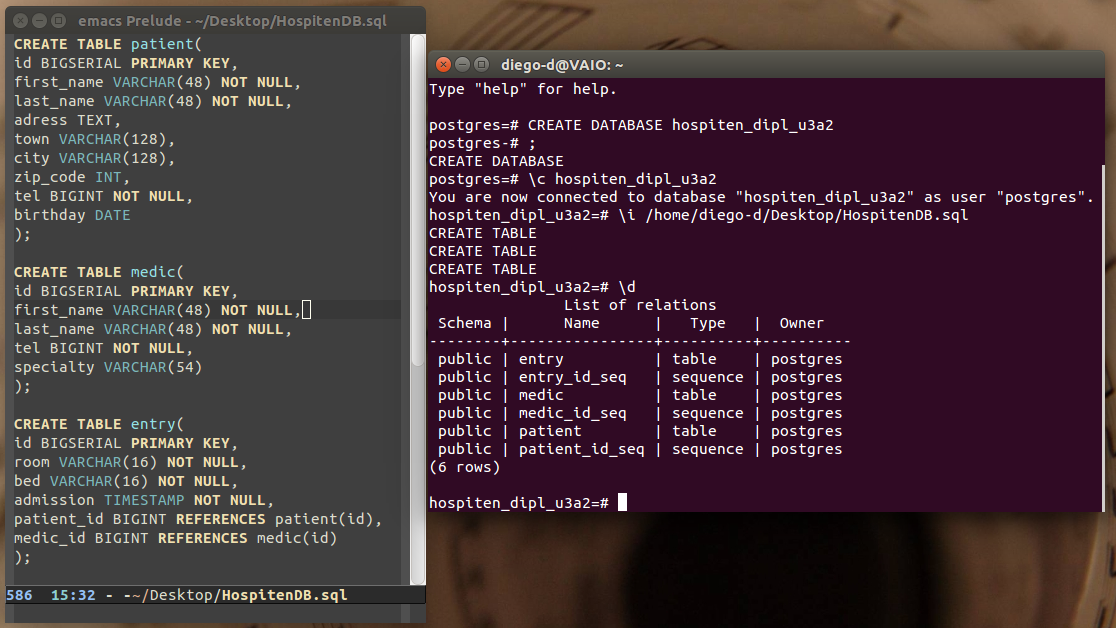
\includegraphics[width=0.8\textwidth]{./tables}~\\[1cm]
	\end{center}
	\begin{center}
	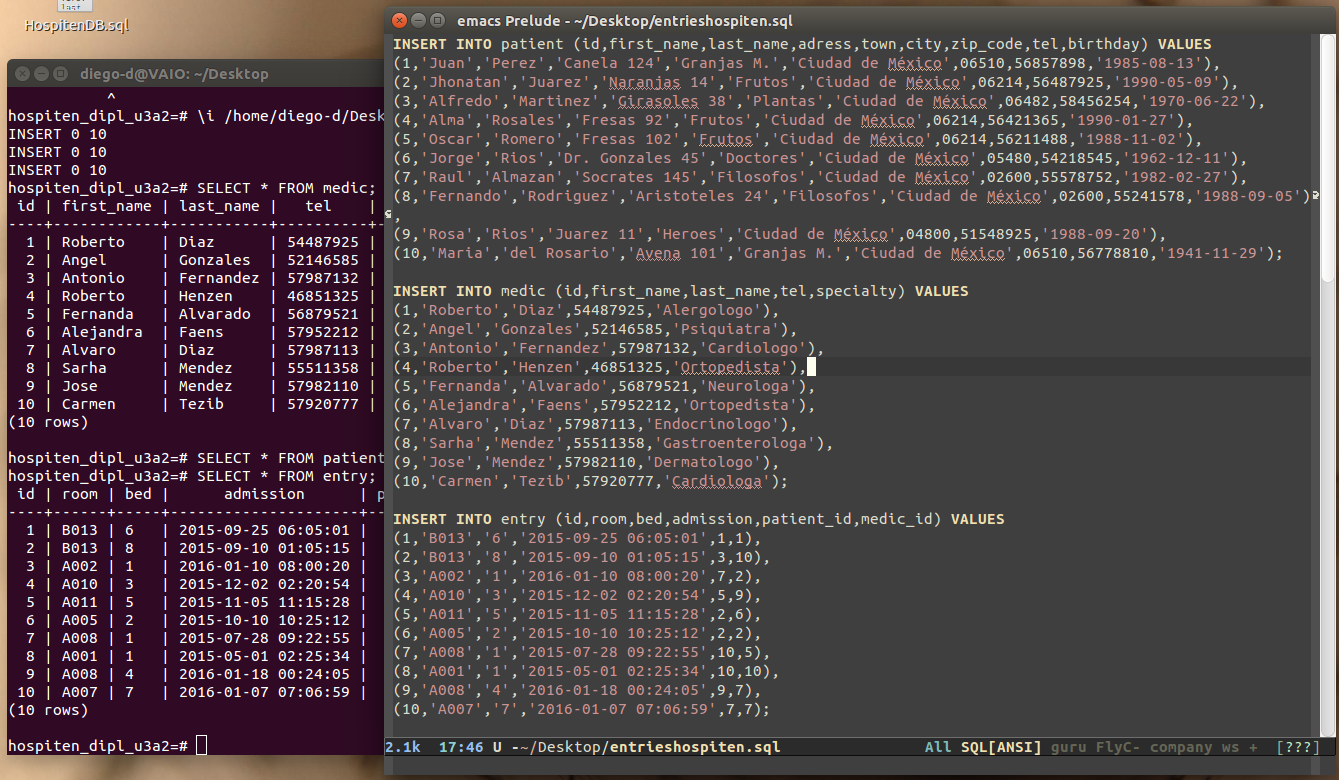
\includegraphics[width=0.8\textwidth]{./entries}~\\[1cm]
	\end{center}
	Aquí se muestra las instrucciones SQL con sentencias de DDL para la creación de tablas, y en la segunda imagen se muestra la entrada de 10 registros.
	
	\section{Vista DB}
	\begin{center}
	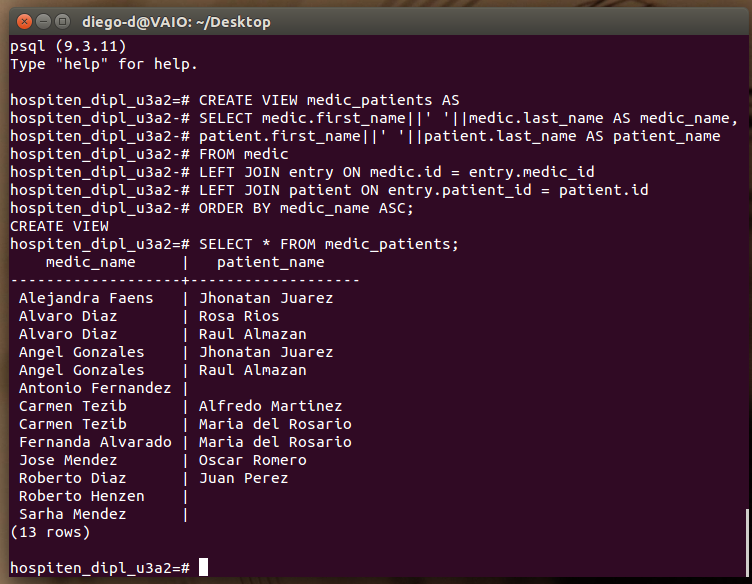
\includegraphics[width=0.8\textwidth]{./view}~\\[1cm]
	\end{center}
	En esta imagen se observa la creación de la vista, que en suma empareja médicos y sus pacientes tomando como referencia la tabla entry. Se realizan 2 LEFT JOIN, el primero para sacar el conjunto de médicos y los datos de las entradas de los pacientes, el segundo es para obtener el conjunto de lo anterior con los pacientes que aparecen este anterior conjunto. Después se hace una consulta para verificar que se haya creado correctamente la vista.
	
	\section{Conclusión}
	Es importante conocer y hacer uso de las Views ya que nos permiten ahorrarnos el usar sentencias largas o para conocer un dato especifico que involucra otros datos sensibles, pero sin mostrar estos. En el uso del modelo relacional. es mas facil trasladarlo a DDL por que este ya contiene las especificaciones, tablas, columnas, tipos de dato, relaciones, etc.
	
	\pagebreak
	\begin{thebibliography}{9}	
	
	\bibitem{psqldocs} The PostgreSQL Development Team. 
		\emph{PostgreSQL 7.0 Docs}. PostgreSQL, [Disponible en: http://www.postgresql.org/docs/7.0/static/postgres.htm].
	
		\bibitem{rrhopkins} Robert J. Robbins. 
		\emph{Database Fundamentals}. Johns Hopkins University, [Disponible en: http://www.esp.org/db-fund.pdf].
		
		\bibitem{elmasriynavathe} Ramez Elmasri and Shamkant Navathe. 
		\emph{Fundamentals of Database Systems}. Pearson Education, [Disponible en: http://tinman.cs.gsu.edu/~raj/4710/f11/Ch01.pdf].

	\end{thebibliography}

\end{document}
